\documentclass[a4paper,12pt]{article}
\usepackage[utf8]{ inputenc}
\usepackage[ngerman]{babel}
\usepackage[a4paper, left=2.5cm, right=2.5cm]{geometry}
\usepackage{graphicx}
\usepackage{subcaption}
\usepackage{fancyhdr}
\usepackage{pdfpages}
\usepackage{listings}
\usepackage{hyperref}
\usepackage[official]{eurosym}
\usepackage{float}

\pagestyle{fancy}
\lstset{
	language=Matlab,
	breaklines=true,
	morekeywords={matlab2tikz},
	keywordstyle=\color{blue},
	morekeywords=[2]{1}, keywordstyle=[2]{\color{black}},
	identifierstyle=\color{black},
	stringstyle=\color{mylilas},
	commentstyle=\color{mygreen},
	showstringspaces=false,
	mathescape=true
	emph=[1]{for,end,break},emphstyle=[1]\color{red},
}

\lhead{PV im Stromsystem – Strommarkt}
\chead{}
\rhead{Gruppe D}

\begin{document}
	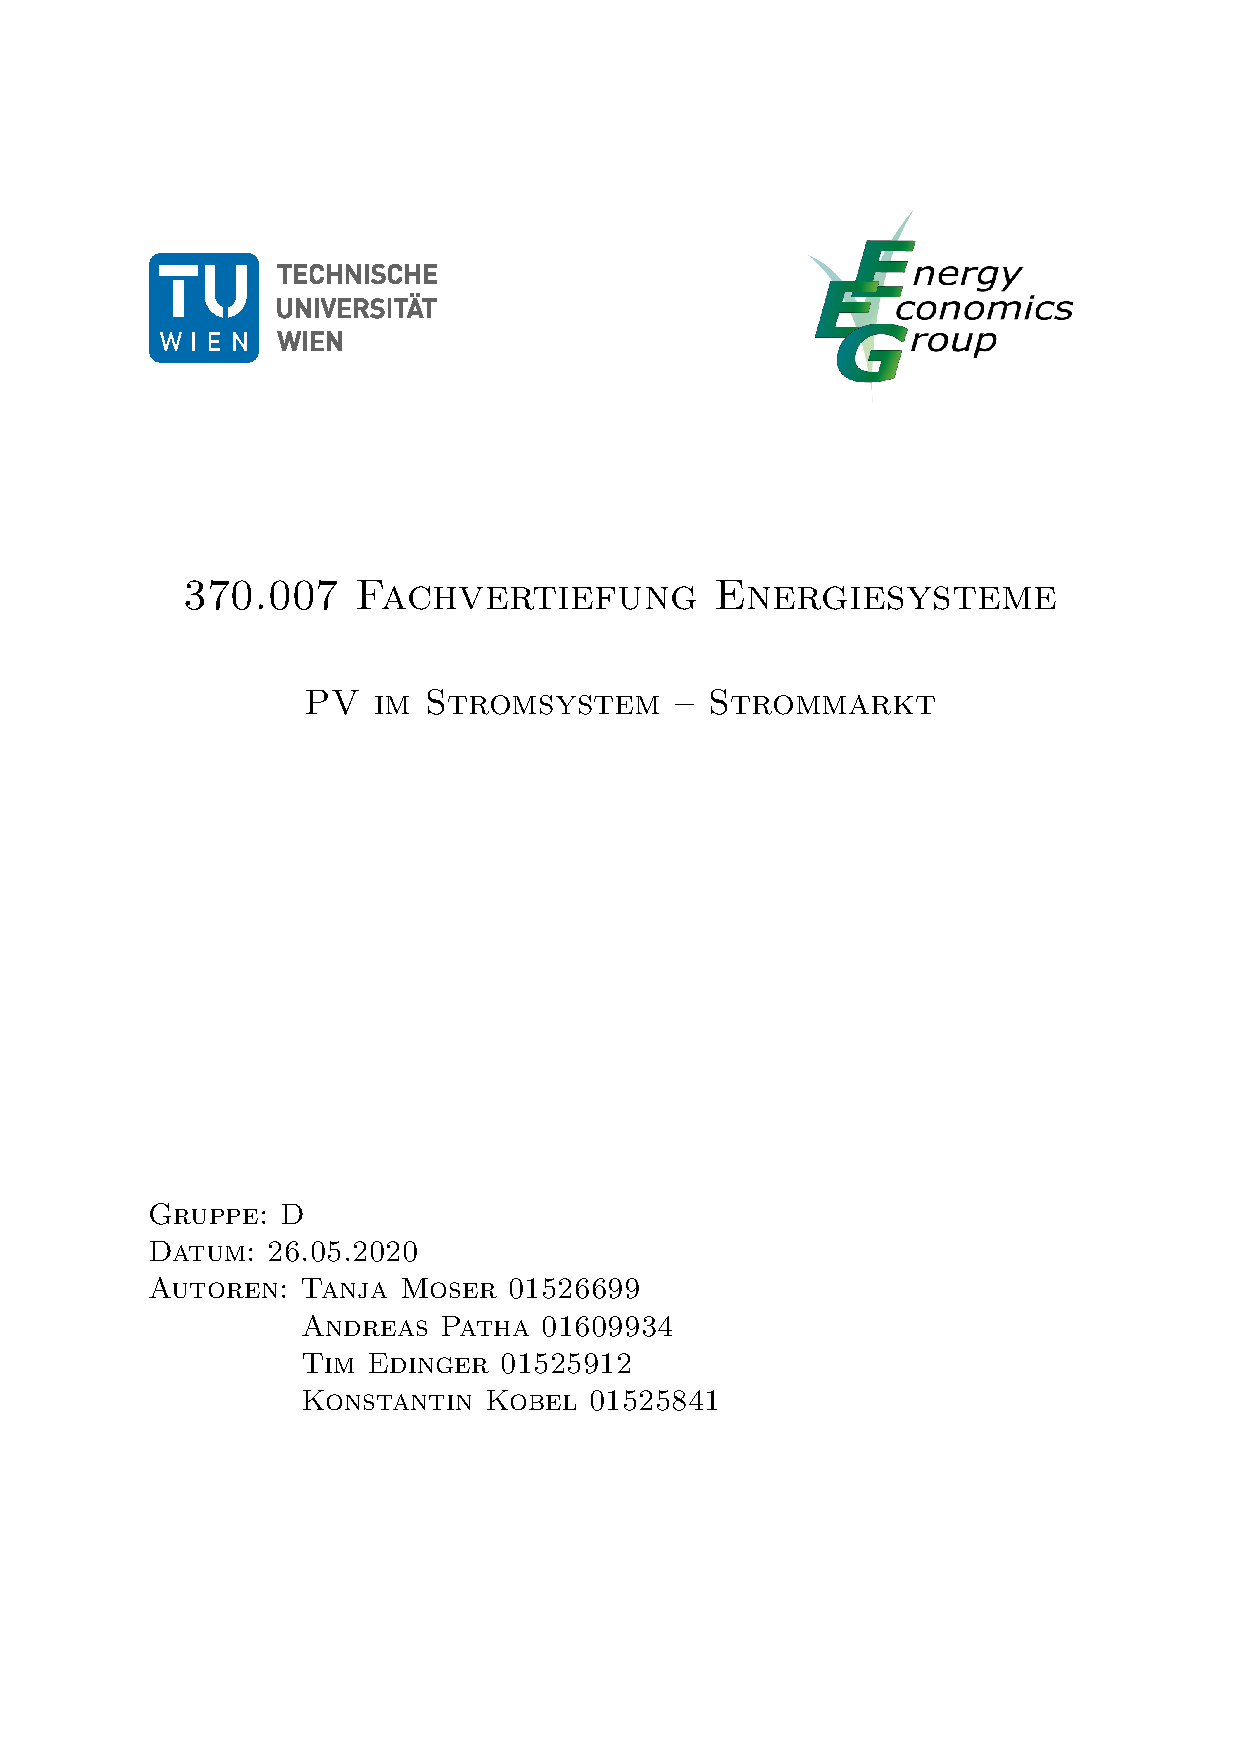
\includepdf{Protokoll_titlepage.pdf}

	\newpage
	\tableofcontents

	\newpage
	\section{Aufgabenstellung}
	\label{sec:Aufgabenstellung}
	
	\section{Berechnungen}
	\label{sec:Berechnungen}
	
	\section{Ergebnisse}
	\label{sec:Ergebnisse}
	
	\newpage
	\listoffigures
\end{document}